\documentclass[../../main.tex]{subfiles}
\begin{document}

{\bf [解]}
\paragraph{(1)}

$f(x)$は最大でも$3$次の関数である．
まず$a\neq 0$の場合，すなわち$f(x)$が三次関数の場合を考える．
(イ)，(ロ)および因数定理から，
\begin{align}
  f(x) = a(x+1)(x-1)(x-\alpha) \quad (\alpha \in \mathbb{R}) \label{eq:1}
\end{align}
と書ける．そこで以下，(ハ)の条件について考える．絶対値を外すと
\begin{align}
  \begin{cases}
    f(x) \ge 1 - x \iff a(x+1)(x-\alpha)(x-1) \ge -(x-1) & (0 \le x \le 1) \\
    f(x) \ge 1+x \iff a(x-1)(x-\alpha)(x+1) \ge (x+1)    & (-1 \le x \le 0)
  \end{cases}
\end{align}
である．これらは$x=\pm 1$では自動で満たされ，それ以外の点では$x-1,x+1$で両辺を割って
\begin{align}
  &
  \begin{cases}
    a(x+1)(x-\alpha) \le -1 & (0 \le x < 1) \\
    a(x-1)(x-\alpha) \le 1  & (-1 < x \le 0)
  \end{cases} \\
  \therefore
  &
  \begin{cases}
    g(x) \equiv a x^2 + a(1-\alpha) x - a\alpha + 1 \le 0 & (0 \le x < 1) \\
    h(x) \equiv a x^2 - a(1+\alpha) x + a\alpha - 1 \ge 0 & (-1 < x \le 0)
  \end{cases} \label{eq:2}
\end{align}
となる．以下これを満たすような$a,\alpha$の条件を考えよう．
今は$a\neq 0$の場合を考えているので$g(x),h(x)$はともに二次関数である．
$a$の正負によって場合分けする．

\subparagraph{$1^{\circ}$ $a>0$の時}

\begin{figure}[htb]
  \centering
  % =========================================================
  % (a) g(x) <= 0 on [0, 1)
  % =========================================================
  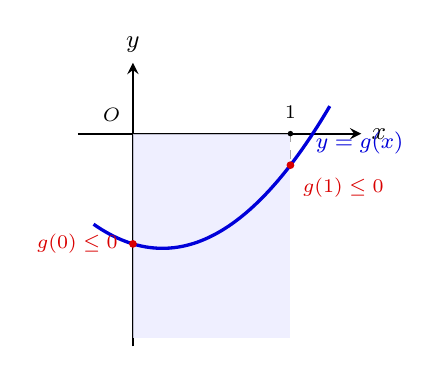
\begin{tikzpicture}[scale=2.0, >=stealth, every node/.style={font=\small}]

    % 座標軸
    \draw[->, thick] (-0.35, 0) -- (1.45, 0) node[right] {$x$};
    \draw[->, thick] (0, -1.35) -- (0, 0.45) node[above] {$y$};
    \node[above left=1pt, font=\scriptsize] at (0, 0) {$O$};

    % 注目区間 [0, 1] の背景帯
    \fill[blue!8, opacity=0.8] (0, -1.3) rectangle (1.0, 0);

    % g(x) のプロット (下に凸、両端 g(0) <= 0, g(1) <= 0)
    % 例: g(x) = 1.2*x^2 - 0.4*x - 0.6  (g(0) = -0.6, g(1) = 0.2 とならないよう g(1) <= 0 に調整)
    % 例: g(x) = 0.8*x^2 - 0.3*x - 0.7  => g(0)=-0.7, g(1)=-0.2
    \draw[very thick, blue!85!black, domain=-0.25:1.25, samples=60]
    plot (\x, {0.8*\x*\x - 0.3*\x - 0.7});
    \node[blue!85!black, font=\footnotesize, right] at (1.1, {0.8*1.1*1.1 - 0.3*1.1 - 0.7}) {$y = g(x)$};

    % 端点 x = 1 の補助線
    \draw[dashed, gray!70] (1.0, 0) -- (1.0, -0.2);
    \fill (1.0, 0) circle (0.5pt) node[above=2pt, font=\scriptsize] {$1$};

    % 端点での値 g(0), g(1)
    \fill[red!85!black] (0, -0.7) circle (0.7pt) node[left=2pt, font=\scriptsize, red!85!black] {$g(0) \le 0$};
    \fill[red!85!black] (1.0, -0.2) circle (0.7pt) node[below right=1pt, font=\scriptsize, red!85!black] {$g(1) \le 0$};

  \end{tikzpicture}
  \caption{$a>0$ における2次関数 $g(x) \le 0$ ($0 \le x < 1$) の条件}
  \label{fig:quadratic_conditions_case1}
\end{figure}

まず$g(x)$についての条件は
\begin{align}
  g(0) \le 0 \land g(1) \le 0 \\
  \therefore
  1-a\alpha \le 0 \land 2a-2a\alpha+1 \le 0 \label{eq:3}
\end{align}
である．

\begin{figure}[htb]
  \centering
  % =========================================================
  % (a) 軸が区間内にある場合: -1 <= (alpha+1)/2 <= 0
  % =========================================================
  \begin{tikzpicture}[scale=2.0, >=stealth, every node/.style={font=\small}]

    % 座標軸
    \draw[->, thick] (-1.45, 0) -- (0.55, 0) node[right] {$x$};
    \draw[->, thick] (0, -0.3) -- (0, 1.45) node[above] {$y$};
    \node[below right=1pt, font=\scriptsize] at (0, 0) {$O$};

    % 注目区間 [-1, 0] の背景
    \fill[orange!12, opacity=0.7] (-1.0, 0) rectangle (0, 1.3);

    % h(x) のプロット (軸が区間内 x0 = -0.45 にあり、頂点の y 座標 >= 0)
    % h(x) = 1.6*(x + 0.45)^2 + 0.15
    \draw[very thick, orange!90!black, domain=-1.15:0.25, samples=60]
    plot (\x, {1.6*(\x + 0.45)*(\x + 0.45) + 0.15});
    \node[orange!90!black, font=\footnotesize, left] at (-1.05, 0.95) {$y = h(x)$};

    % 軸の位置 x = -0.45
    \draw[dashed, gray!70] (-0.45, -0.15) -- (-0.45, 1.15);
    \node[gray!80!black, font=\scriptsize, below] at (-0.45, -0.15) {軸 $x_0$};

    % 頂点 (最小値 >= 0)
    \fill[red!85!black] (-0.45, 0.15) circle (0.7pt);
    \node[red!85!black, font=\scriptsize, above=2pt] at (-0.45, 0.15) {頂点 $\ge 0$ ($D/4 \le 0$)};

    % 区間の両端 x = -1, 0
    \draw[dashed, gray!50] (-1.0, 0) -- (-1.0, {1.6*(-0.55)*(-0.55) + 0.15});
    \fill (-1.0, 0) circle (0.5pt) node[below=2pt, font=\scriptsize] {$-1$};
    \fill (0, 0) circle (0.5pt);

  \end{tikzpicture}
  \hspace{0.8cm}
  % =========================================================
  % (b) 軸が区間外にある場合: (alpha+1)/2 <= -1 または 0 <= (alpha+1)/2
  % =========================================================
  \begin{tikzpicture}[scale=2.0, >=stealth, every node/.style={font=\small}]

    % 座標軸
    \draw[->, thick] (-1.45, 0) -- (0.65, 0) node[right] {$x$};
    \draw[->, thick] (0, -0.3) -- (0, 1.45) node[above] {$y$};
    \node[below right=1pt, font=\scriptsize] at (0, 0) {$O$};

    % 注目区間 [-1, 0] の背景
    \fill[orange!12, opacity=0.7] (-1.0, 0) rectangle (0, 1.3);

    % h(x) のプロット (軸が右側の区間外 x0 = 0.35 にあり、単調減少で区間内 >= 0)
    % h(x) = 1.0*(x - 0.35)^2 + 0.08
    \draw[very thick, orange!90!black, domain=-1.15:0.55, samples=60]
    plot (\x, {1.0*(\x - 0.35)*(\x - 0.35) + 0.08});
    \node[orange!90!black, font=\footnotesize, right] at (0.42, 0.45) {$y = h(x)$};

    % 軸の位置 x = 0.35 (区間外)
    \draw[dashed, gray!70] (0.35, -0.15) -- (0.35, 0.95);
    \node[gray!80!black, font=\scriptsize, below] at (0.35, -0.15) {軸 $x_0 \ge 0$};

    % 区間端点 x = -1, 0 での値
    \pgfmathsetmacro{\yLeft}{1.0*(-1.35)*(-1.35) + 0.08}
    \pgfmathsetmacro{\yRight}{1.0*(-0.35)*(-0.35) + 0.08}

    \draw[dashed, gray!50] (-1.0, 0) -- (-1.0, \yLeft);
    \fill (-1.0, 0) circle (0.5pt) node[below=2pt, font=\scriptsize] {$-1$};
    \fill[red!85!black] (-1.0, \yLeft) circle (0.7pt) node[above left=1pt, font=\scriptsize, red!85!black] {$h(-1) \ge 0$};
    \fill[red!85!black] (0, \yRight) circle (0.7pt) node[above right=1pt, font=\scriptsize, red!85!black] {$h(0) \ge 0$};

  \end{tikzpicture}
  \caption{$a>0$ における $h(x) \ge 0$（$-1 < x \le 0$）の軸の位置による条件の分類}
  \label{fig:h_quadratic_axis_cases}
\end{figure}

ついで$h(x)$についての条件は軸の位置 $x = \dfrac{\alpha+1}{2}$ で場合分けする．
すなわち，軸が$[-1,0]$に含まれていれば$h(x)$の判別式($D'$)が非正であればよく，軸が区間の外にあれば両端で$h(x)$が正であれば良い：
\begin{align}
  &
  \begin{cases}
    D'\le 0 & \left(-1 \le \dfrac{\alpha+1}{2} \le 0\right) \\
    g(0)\ge 0 \land g(-1)\ge 0 & \text{otherwise}
  \end{cases} \\
  \therefore
  &
  \begin{cases}
    a^2(\alpha+1)^2-4a(a\alpha-1)\ge 0 & \left(-1 \le \dfrac{\alpha+1}{2} \le 0\right) \\
    g(0)\ge 0 \land g(-1)\ge 0 & \text{otherwise}
  \end{cases} \\
  \therefore
  &
  \begin{cases}
    a\left[a(\alpha-1)^2+4\right]\ge 0       & -1 \le \dfrac{\alpha+1}{2} \le 0 \\
    2a+2a\alpha-1\ge 0 \land a\alpha-1 \ge 0 & \text{otherwise}
  \end{cases}
\end{align}
となる．ここで$a>0$より$a\left[a(\alpha-1)^2+4\right]>0$だから，第一式を満たす$(a,\alpha)$はなく，第二式だけを考えれば良い．
\begin{align}
  2a+2a\alpha-1\ge 0 \land a\alpha-1 \ge 0 \quad \left(\dfrac{\alpha+1}{2} \le -1, 0 \le \dfrac{\alpha+1}{2}\right) \label{eq:4}
\end{align}
である．

\cref{eq:3,eq:4}をまとめて，(ハ)を満たすような$a,\alpha$の条件は
\begin{align}
  &
  \begin{cases}
    1-a\alpha \le 0 \\
    2a-2a\alpha+1 \le 0 \\
    2a+2a\alpha-1 \ge 0 \\
    \dfrac{\alpha+1}{2} \le -1 \\
    0 \le \dfrac{\alpha+1}{2}
  \end{cases} \\
  \therefore
  &
  \begin{cases}
    a\alpha \ge 1 \\
    2a-2a\alpha+1 \le 0 \\
    2a+2a\alpha-1 \ge 0 \\
    \alpha \le -3, -1 \le \alpha
  \end{cases}
\end{align}
である．$a>0$に注意してこれを$\alpha$について整理すると
\begin{align}
  \begin{cases}
    \alpha \ge \dfrac{1}{a} \\
    \alpha \ge \dfrac{2a+1}{2a} \\
    \alpha \ge \dfrac{-2a+1}{2a} \\
    \alpha \le -3, -1 \le \alpha
  \end{cases}
\end{align}
であり，図示すると下図の斜線部のようになる．

\begin{figure}[htb]
  \centering
  \begin{tikzpicture}[scale=2.2, >=stealth, every node/.style={font=\small}]

    % --- 1. 共通領域の斜線ハッチング ---
    % 条件 (a > 0):
    % alpha >= 1/a, alpha >= 1 + 1/(2a), alpha >= -1 + 1/(2a), alpha <= -3 または alpha >= -1
    % a > 0 では 1/a > 1 + 1/(2a) <=> 2 > 2a + 1 <=> a < 1/2
    % したがって上境界は:
    %   0 < a <= 1/2: alpha = 1/a
    %   a >= 1/2    : alpha = 1 + 1/(2a)
    % さらに alpha >= -1 より、上境界より上の領域全体が解となる
    \fill[pattern=north east lines, pattern color=blue!60, opacity=0.8]
    plot[domain=0.25:0.5, samples=50] (\x, {1.0/\x})
    -- plot[domain=0.5:2.5, samples=60] (\x, {1.0 + 1.0/(2.0*\x)})
    -- (2.5, 4.2) -- (0.25, 4.2)
    -- cycle;

    % --- 2. 座標軸 ---
    \draw[->, thick] (-0.3, 0) -- (2.8, 0) node[right] {$a$};
    \draw[->, thick] (0, -3.6) -- (0, 4.3) node[above] {$\alpha$};
    \node[below left=2pt] at (0, 0) {$O$};

    % --- 3. 境界となる曲線・直線群 ---
    % (i) alpha = 1/a (青太線)
    \draw[very thick, blue!85!black, domain=0.24:2.5, samples=80]
    plot (\x, {1.0/\x});
    \node[blue!85!black, font=\footnotesize, right] at (2.2, 0.45) {$\alpha = \frac{1}{a}$};

    % (ii) alpha = (2a+1)/(2a) = 1 + 1/(2a) (赤太線)
    \draw[very thick, red!85!black, domain=0.2:2.5, samples=80]
    plot (\x, {1.0 + 1.0/(2.0*\x)});
    \node[red!85!black, font=\footnotesize, right] at (2.2, 1.35) {$\alpha = \frac{2a+1}{2a}$};

    % (iii) alpha = (-2a+1)/(2a) = -1 + 1/(2a) (緑線・細線)
    \draw[thick, teal!85!black, domain=0.2:2.5, samples=80]
    plot (\x, {-1.0 + 1.0/(2.0*\x)});
    \node[teal!85!black, font=\footnotesize, right] at (2.2, -0.65) {$\alpha = \frac{-2a+1}{2a}$};

    % (iv) 水平境界線 alpha = -1, alpha = -3
    \draw[dashed, gray!70] (0, -1) -- (2.5, -1) node[right, font=\scriptsize] {$\alpha = -1$};
    \draw[dashed, gray!70] (0, -3) -- (2.5, -3) node[right, font=\scriptsize] {$\alpha = -3$};

    % 水平線 alpha = 1 (漸近線参考)
    \draw[dotted, gray!50] (0, 1) -- (2.5, 1) node[right, font=\tiny] {$\alpha = 1$};

    % --- 4. 交点 (1/2, 2) と座標目盛り ---
    % 1/a と (2a+1)/(2a) の交点は a = 1/2, alpha = 2
    \draw[dashed, gray!60] (0.5, 0) -- (0.5, 2) -- (0, 2);
    \fill (0.5, 2) circle (0.7pt);
    \node[above right=1pt, font=\scriptsize] at (0.5, 2) {$\left(\frac{1}{2}, 2\right)$};

    % 軸上の目盛り
    \fill (0.5, 0) circle (0.4pt) node[below=2pt, font=\scriptsize] {$\frac{1}{2}$};
    \fill (0, 2) circle (0.4pt) node[left=2pt, font=\scriptsize] {$2$};
    \fill (0, 1) circle (0.4pt) node[left=2pt, font=\scriptsize] {$1$};
    \fill (0, -1) circle (0.4pt) node[left=2pt, font=\scriptsize] {$-1$};
    \fill (0, -3) circle (0.4pt) node[left=2pt, font=\scriptsize] {$-3$};

    % --- 5. 領域注記 ---
    \node[draw=blue!85!black, fill=white, rounded corners=2pt, inner sep=3pt, font=\footnotesize, align=center]
    at (1.5, 3.2) {求める領域（斜線部）\\[2pt]
      $
      \begin{cases}
        \alpha \ge \frac{1}{a} & \left(0 < a \le \frac{1}{2}\right) \\[4pt]
        \alpha \ge \frac{2a+1}{2a} & \left(a \ge \frac{1}{2}\right)
    \end{cases}$};

  \end{tikzpicture}
  \caption{$a > 0$ における連立不等式を満たす $(a, \alpha)$ 平面の領域}
  \label{fig:a_alpha_region_positive}
\end{figure}

従って求める条件は
\begin{align}
  \begin{cases}
    \alpha \ge \dfrac{1}{a} & \left(0 < a \le \dfrac{1}{2}\right) \\[4pt]
    \alpha \ge \dfrac{2a+1}{2a} & \left(a \ge \dfrac{1}{2}\right)
  \end{cases} \label{eq:5}
\end{align}
である．

\subparagraph{$2^{\circ}$ $a<0$の時}

$g(x)$の条件は$g(x)$の軸の位置$x=\dfrac{\alpha-1}{2}$で場合分けする．
$g(x)=0$の判別式$D$とおく．
\begin{align}
  &
  \begin{cases}
    D \le 0 & \left(0 \le \dfrac{\alpha-1}{2} \le 1\right) \\
    g(0) \le 0 \land g(1) \le 0 & \text{otherwise}
  \end{cases} \\
  \therefore
  &
  \begin{cases}
    a^2(1-\alpha)^2-4a(1-a\alpha)\le 0 & \left(0 \le \dfrac{\alpha-1}{2} \le 1\right) \\
    a\alpha-1 \le 0 \land 2a-2a\alpha + 1 \le 0 & \text{otherwise}
  \end{cases} \\
  \therefore
  &
  \begin{cases}
    a\left[a(\alpha+1)^2-4\right] \le 0 & \left(0 \le \dfrac{\alpha-1}{2} \le 1\right) \\
    a\alpha-1 \le 0 \land 2a-2a\alpha + 1 \le 0 & \text{otherwise}
  \end{cases}
\end{align}
である．$a<0$だから$a\left[a(\alpha+1)^2-4\right]>0$であり，第一式を満たす$(a,\alpha)$は存在しないから第二式だけ考えればよく，
\begin{align}
  a\alpha-1 \le 0 \land 2a-2a\alpha+1 \le 0 \quad \left(\dfrac{\alpha-1}{2} \le 0, 1 \le \dfrac{\alpha-1}{2}\right) \label{eq:6}
\end{align}
である．

次に$h(x)$の条件は
\begin{align}
  & g(-1) \ge 0 \land g(0) \ge 0 \\
  \therefore
  & 2a+2a\alpha-1\ge 0 \land a\alpha-1 \ge 0 \label{eq:7}
\end{align}
である．

\cref{eq:6,eq:7}をまとめて
\begin{align}
  &
  \begin{cases}
    a\alpha \ge 1 \\
    2a-2a\alpha+1 \le 0 \\
    2a+2a\alpha-1 \ge 0 \\
    \dfrac{\alpha-1}{2} \le 0, 1 \le \dfrac{\alpha-1}{2}
  \end{cases} \\
  \therefore
  &
  \begin{cases}
    a\alpha \ge 1 \\
    2a-2a\alpha+1 \le 0 \\
    2a+2a\alpha-1 \ge 0 \\
    \alpha \le 1, 3 \le \alpha
  \end{cases}
\end{align}
である．$a<0$に注意して$\alpha$について整理すると
\begin{align}
  \begin{cases}
    \alpha \le \dfrac{1}{a} \\
    \alpha \ge \dfrac{2a+1}{2a} \\
    \alpha \le \dfrac{-2a+1}{2a}
    \alpha \le 1, 3 \le \alpha
  \end{cases}
\end{align}
であり，図示すると下図の斜線部のようになる．

\begin{figure}[htb]
  \centering
  \begin{tikzpicture}[scale=2.2, >=stealth, every node/.style={font=\small}]

    % --- 1. 共通領域の斜線ハッチング ---
    % 条件 (a < 0):
    % alpha <= 1/a, alpha >= 1 + 1/(2a), alpha <= -1 + 1/(2a), alpha <= 1 または 3 <= alpha
    % a < 0 では常に 1 + 1/(2a) <= alpha <= -1 + 1/(2a) は成立しないため、
    % 境界曲線:
    %   -1/2 <= a < 0: alpha <= 1/a
    %   a <= -1/2    : alpha <= -1 + 1/(2a) = (-2a+1)/(2a)
    % さらに alpha <= 1 より、下境界より下の領域全体が解となる
    \fill[pattern=north east lines, pattern color=blue!60, opacity=0.8]
    plot[domain=-2.5:-0.5, samples=60] (\x, {-1.0 + 1.0/(2.0*\x)})
    -- plot[domain=-0.5:-0.25, samples=50] (\x, {1.0/\x})
    -- (-0.25, -4.2) -- (-2.5, -4.2)
    -- cycle;

    % --- 2. 座標軸 ---
    \draw[->, thick] (-2.8, 0) -- (0.5, 0) node[right] {$a$};
    \draw[->, thick] (0, -4.3) -- (0, 3.6) node[above] {$\alpha$};
    \node[below right=2pt] at (0, 0) {$O$};

    % --- 3. 境界となる曲線・直線群 ---
    % (i) alpha = 1/a (青太線)
    \draw[very thick, blue!85!black, domain=-2.5:-0.24, samples=80]
    plot (\x, {1.0/\x});
    \node[blue!85!black, font=\footnotesize, left] at (-2.3, -0.45) {$\alpha = \frac{1}{a}$};

    % (ii) alpha = (-2a+1)/(2a) = -1 + 1/(2a) (赤太線)
    \draw[very thick, red!85!black, domain=-2.5:-0.2, samples=80]
    plot (\x, {-1.0 + 1.0/(2.0*\x)});
    \node[red!85!black, font=\footnotesize, left] at (-2.3, -1.4) {$\alpha = \frac{-2a+1}{2a}$};

    % (iii) alpha = (2a+1)/(2a) = 1 + 1/(2a) (緑線・細線)
    \draw[thick, teal!85!black, domain=-2.5:-0.2, samples=80]
    plot (\x, {1.0 + 1.0/(2.0*\x)});
    \node[teal!85!black, font=\footnotesize, left] at (-2.3, 0.6) {$\alpha = \frac{2a+1}{2a}$};

    % (iv) 水平境界線 alpha = 1, alpha = 3
    \draw[dashed, gray!70] (-2.5, 1) -- (0, 1) node[right, font=\scriptsize] {$\alpha = 1$};
    \draw[dashed, gray!70] (-2.5, 3) -- (0, 3) node[right, font=\scriptsize] {$\alpha = 3$};

    % 水平線 alpha = -1 (漸近線参考)
    \draw[dotted, gray!50] (-2.5, -1) -- (0, -1) node[right, font=\tiny] {$\alpha = -1$};

    % --- 4. 交点 (-1/2, -2) と座標目盛り ---
    % 1/a と (-2a+1)/(2a) の交点は a = -1/2, alpha = -2
    \draw[dashed, gray!60] (-0.5, 0) -- (-0.5, -2) -- (0, -2);
    \fill (-0.5, -2) circle (0.7pt);
    \node[below left=1pt, font=\scriptsize] at (-0.5, -2) {$\left(-\frac{1}{2}, -2\right)$};

    % 軸上の目盛り
    \fill (-0.5, 0) circle (0.4pt) node[above=2pt, font=\scriptsize] {$-\frac{1}{2}$};
    \fill (0, -2) circle (0.4pt) node[right=2pt, font=\scriptsize] {$-2$};
    \fill (0, -1) circle (0.4pt) node[right=2pt, font=\scriptsize] {$-1$};
    \fill (0, 1)  circle (0.4pt) node[right=2pt, font=\scriptsize] {$1$};
    \fill (0, 3)  circle (0.4pt) node[right=2pt, font=\scriptsize] {$3$};

    % --- 5. 領域注記 ---
    \node[draw=blue!85!black, fill=white, rounded corners=2pt, inner sep=3pt, font=\footnotesize, align=center]
    at (-1.5, -3.2) {求める領域（斜線部）\\[2pt]
      $
      \begin{cases}
        \alpha \le \frac{1}{a} & \left(-\frac{1}{2} \le a < 0\right) \\[4pt]
        \alpha \le \frac{-2a+1}{2a} & \left(a \le -\frac{1}{2}\right)
    \end{cases}$};

  \end{tikzpicture}
  \caption{$a < 0$ における連立不等式を満たす $(a, \alpha)$ 平面の領域}
  \label{fig:a_alpha_region_negative}
\end{figure}

従って求める条件は
\begin{align}
  \begin{cases}
    \alpha \le \dfrac{1}{a} & \left(-\dfrac{1}{2} \le a < 0\right) \\[4pt]
    \alpha \le \dfrac{-2a+1}{2a} & \left(a \le -\dfrac{1}{2}\right)
  \end{cases} \label{eq:8}
\end{align}

\casesend

以上$1^\circ, 2^\circ$ をまとめると
\begin{align}
  \begin{cases}
    \alpha \le \dfrac{1}{a} & \left(-\dfrac{1}{2} \le a < 0\right) \\[4pt]
    \alpha \le \dfrac{-2a+1}{2a} & \left(a \le -\dfrac{1}{2}\right) \\[4pt]
    \alpha \ge \dfrac{1}{a} & \left(0 < a \le \dfrac{1}{2}\right) \\[4pt]
    \alpha \ge \dfrac{2a+1}{2a} & \left(a \ge \dfrac{1}{2}\right)
  \end{cases} \label{eq:9}
\end{align}
である．

ここで，$f(x) = a(x^2-1)(x-\alpha) = a(x^3 - \alpha x^2 - x + \alpha)$ だから，
係数比較して
\begin{align}
  b = -d = -a\alpha, \quad c = -a \label{eq:10}
\end{align}
である．従って\cref{eq:9}に代入して$\alpha$を消去すると
\begin{align}
  \begin{cases}
    2b \le 2a-1 & \left(a \le -\dfrac{1}{2}\right) \\[4pt]
    b  \le -1     & \left(-\dfrac{1}{2} \le a < \dfrac{1}{2}, a\neq 0\right) \\[4pt]
    2b \le -2a-1  & \left(a \ge \dfrac{1}{2}\right) \\[4pt]
    b = -d, c = -a
  \end{cases} \label{eq:11}
\end{align}
である．

さて次に$a=0$ の時を考える．
$f(x)$ が $1$ 次以下だと(イ)(ロ)の両方を同時に満たせず不適なので $b \neq 0$ のもとで考えればよく，(イ)(ロ)から
\begin{align}
  f(x) = b(x^2-1)
\end{align}
とおける．すなわち$a=c=0,b=-d=1$である．

\begin{figure}[htb]
  \centering
  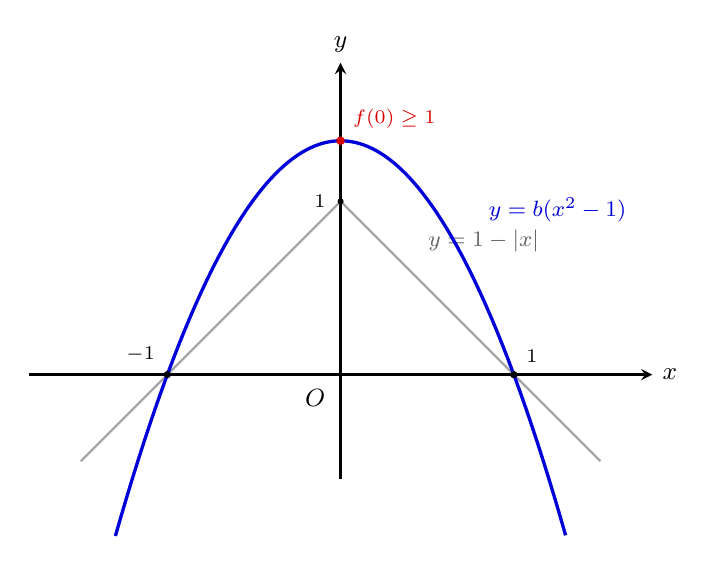
\begin{tikzpicture}[scale=2.2, >=stealth, every node/.style={font=\small}]

    % --- 1. 座標軸 ---
    \draw[->, thick] (-1.8, 0) -- (1.8, 0) node[right] {$x$};
    \draw[->, thick] (0, -0.6) -- (0, 1.8) node[above] {$y$};
    \node[below left=2pt] at (0, 0) {$O$};

    % --- 2. 条件の境界線: 折れ線 y = 1 - |x| ---
    \draw[thick, gray!70] (-1.5, -0.5) -- (-1.0, 0) -- (0, 1.0) -- (1.0, 0) -- (1.5, -0.5);
    \node[gray!80!black, font=\footnotesize, above right] at (0.45, 0.65) {$y = 1 - |x|$};

    % --- 3. 放物線 f(x) = b(x^2 - 1) (例: b = -1.35 => f(0) = 1.35 >= 1) ---
    \draw[very thick, blue!85!black, domain=-1.3:1.3, samples=80]
    plot (\x, {-1.35*(\x*\x - 1.0)});
    \node[blue!85!black, font=\footnotesize, right] at (0.8, 0.95) {$y = b(x^2 - 1)$};

    % --- 4. 頂点 f(0) = -b >= 1 の強調 ---
    \fill[red!85!black] (0, 1.35) circle (0.7pt) node[above right=1pt, font=\scriptsize, red!85!black] {$f(0) \ge 1$};
    \fill (0, 1.0) circle (0.5pt) node[left=2pt, font=\scriptsize] {$1$};

    % --- 5. x 切片 (-1, 0) および (1, 0) ---
    \fill (-1.0, 0) circle (0.6pt) node[above left=1pt, font=\scriptsize] {$-1$};
    \fill (1.0, 0) circle (0.6pt) node[above right=1pt, font=\scriptsize] {$1$};

  \end{tikzpicture}
  \caption{$a=0$ における $f(x) = b(x^2-1)$ と折れ線 $y = 1 - |x|$ の関係}
  \label{fig:case_a0_parabola}
\end{figure}

(ハ)の条件を図形的に考えると，$f(x)$が二次関数だから条件は
\begin{align}
  f(0) \ge 1 \iff 1+b \le 0 \label{eq:12}
\end{align}
である．
従って$a=0$の時は\cref{eq:11}に吸収できて，最終的に求める条件は
\begin{align}
  \begin{cases}
    2b \le 2a-1 & \left(a \le -\dfrac{1}{2}\right) \\[4pt]
    b  \le -1     & \left(-\dfrac{1}{2} \le a < \dfrac{1}{2}\right) \\[4pt]
    2b \le -2a-1  & \left(a \ge \dfrac{1}{2}\right) \\[4pt]
    b = -d, c = -a &
  \end{cases} \label{eq:13}
\end{align}
である．特に$a,b$の条件を図示すると下図の斜線部（境界を含む）である．

\begin{figure}[htb]
  \centering
  \begin{tikzpicture}[scale=2.2, >=stealth, every node/.style={font=\small}]

    % --- 1. 領域の定義と斜線ハッチング ---
    % 条件:
    % 1 + b <= 0  <=>  b <= -1
    % 2a + 2b + 1 <= 0  <=>  b <= -a - 1/2
    % 2a - 2b - 1 >= 0  <=>  b <= a - 1/2
    % これらをまとめた上側境界線:
    %   |a| <= 1/2 のとき: b <= -1 (※解(1)の1+b<=0条件を反映)
    %   a >= 1/2 のとき: b <= -a - 1/2
    %   a <= -1/2 のとき: b <= a - 1/2
    \fill[pattern=north east lines, pattern color=blue!60, opacity=0.75]
    (-1.8, -2.3) -- (-1.8, -2.3)
    -- (-0.5, -1.0) -- (0.5, -1.0)
    -- (1.8, -2.3) -- (1.8, -2.5)
    -- (-1.8, -2.5) -- cycle;

    % --- 2. 座標軸 ---
    \draw[->, thick] (-2.0, 0) -- (2.0, 0) node[right] {$a$};
    \draw[->, thick] (0, -2.6) -- (0, 0.8) node[above] {$b$};
    \node[below left=2pt] at (0, 0) {$O$};

    % --- 3. 境界線 ---
    % 直線 b = -a - 1/2 (2a + 2b + 1 = 0)
    \draw[very thick, red!85!black, domain=-0.2:1.9]
    plot (\x, {-\x - 0.5});
    \node[red!85!black, font=\footnotesize, right] at (1.5, -2.0) {$b = -a - \frac{1}{2}$};

    % 直線 b = a - 1/2 (2a - 2b - 1 = 0)
    \draw[very thick, teal!85!black, domain=-1.9:0.2]
    plot (\x, {\x - 0.5});
    \node[teal!85!black, font=\footnotesize, left] at (-1.5, -2.0) {$b = a - \frac{1}{2}$};

    % 水平境界線 b = -1 (1 + b <= 0)
    \draw[very thick, blue!85!black] (-1.9, -1.0) -- (1.9, -1.0);
    \node[blue!85!black, font=\footnotesize, above right] at (1.0, -1.0) {$b = -1$};

    % 参考補助線 b = -1/2
    \draw[dashed, gray!60] (-1.8, -0.5) -- (1.8, -0.5) node[right, font=\tiny, gray!70!black] {$b = -\frac{1}{2}$};

    % --- 4. 座標補助線・目盛り ---
    % a = 1/2, a = -1/2 の補助線
    \draw[dashed, gray!60] (0.5, 0) -- (0.5, -1.0);
    \draw[dashed, gray!60] (-0.5, 0) -- (-0.5, -1.0);

    \fill (0.5, 0) circle (0.4pt) node[above=2pt, font=\scriptsize] {$\frac{1}{2}$};
    \fill (-0.5, 0) circle (0.4pt) node[above=2pt, font=\scriptsize] {$-\frac{1}{2}$};
    \fill (0, -0.5) circle (0.4pt) node[left=2pt, font=\scriptsize] {$-\frac{1}{2}$};
    \fill (0, -1.0) circle (0.4pt) node[left=2pt, font=\scriptsize] {$-1$};

    % 境界の角（折れ曲がり点）
    \fill (0.5, -1.0) circle (0.6pt);
    \fill (-0.5, -1.0) circle (0.6pt);

  \end{tikzpicture}
  \caption{$(a,b)$ 平面における条件を満たす領域}
  \label{fig:ab_parameter_region}
\end{figure}

\paragraph{(2)}

(1)で求めた$f(x)$のうちで，与えられた定積分
\begin{align}
  I = \int_{-1}^{1}\left[f'(x)-x\right]^2 dx \label{eq:14}
\end{align}
を最小にするものを考える．

(1)から
\begin{align}
  f(x) = ax^3 + bx^2 - ax - b
\end{align}
とおける．一階微分は
\begin{align}
  f'(x) = 3ax^2 + 2bx - a
\end{align}
だから，被積分関数は
\begin{align}
  \{f'(x) - x\}^2
  &= \left[3ax^2 + (2b-1)x - a\right]^2 \\
  &= (3ax^2)^2 + (2b-1)^2 x^2 + a^2 + 2 \Bigl[ 3a(2b-1) x^3 - 3a^2 x^2 - (2b-1)ax \Bigr] \\
  &= 9a^2 x^4 + \Bigl[ (2b-1)^2 - 6a^2 \Bigr] x^2 + a^2 + (\text{奇数次項})
\end{align}
と展開できるから，\cref{eq:14}に代入して
\begin{align}
  I
  &= \int_{-1}^1 \{f'(x) - x\}^2 \, dx \\
  &= 2 \int_0^1 \Bigl( 9a^2 x^4 + \Bigl[ (2b-1)^2 - 6a^2 \Bigr] x^2 + a^2 \Bigr) dx \\
  &= 2 \Bigl[ a^2 \int_0^1 (9x^4 - 6x^2 + 1) dx + (2b-1)^2 \int_0^1 x^2 dx \Bigr] \\
  &= 2 \Bigl[ \dfrac{4}{5} a^2 + \dfrac{1}{3}(2b-1)^2 \Bigr] \label{eq:15}
\end{align}
となる．

(1)の$(a,b)$の動く領域から，$I$が最小になるのは$(a,b)=(0,-1)$の時の$I=6$である．
この時$f(x)$は
\begin{align}
  f(x) = -x^2+1
\end{align}
である．

% TODO: これを考える
% \bigskip\noindent{\bf [解2]} 軽〜く処理するなら…
% (ハ)の条件は $f'(1) \le -1, f'(-1) \ge 1, f(0) \ge 1$ である．

\end{document}
